% !TEX root = ../thesis-example.tex
%
\chapter{Notions et éléments de base de la géométrie digitale}
\label{sec:notions}

\cleanchapterquote{We have seen that computer programming is an art, because it applies accumulated knowledge to the world, because it requires skill and ingenuity, and especially because it produces objects of beauty.}{Jean-Claude Vandamme}{Ma vie, mon œuvre.}

\setcounter{minitocdepth}{3}
\minitoc

\newpage
%
\section{Introduction}
%
Dans ce chapitre, nous allons poser les définissions des éléments dont nous allons nous servir pour la suite de ce document. Cela comprend une introduction à la géométrie différentielle (\RefSection{sec:geo-diff}) permettant de faire le lien entre les mathématiques et nos estimateurs digitaux, ainsi que tout le pipeline permettant d'analyser le comportement d'un estimateur digital (\RefSection{sec:multigrid-convergence-estimator}).
\todoInlineJeremy{faire l'introduction chapitre notions}
% historique geo dis : http://www.citr.auckland.ac.nz/~rklette/talks/01_CP.pdf
%
\section{Notations}
%
Le \RefTable{tab:notations} montre la signification des notations utilisées
dans cette thèse (sauf mention contraire).

\begin{table}[ht]
  \centering
  \caption{Notations utilisées dans cette thèse}
  \label{tab:notations}
    \renewcommand{\arraystretch}{1.1}
  \begin{tabular}{@{}lp{9cm}p{2.5cm}@{}}
    \toprule
    Notation      & Description  & Définition \\ \midrule

    $\R^d$        & Espace euclidien de dimension $d$ & \RefSectionTable{sec:notions} \\
    $\Shapes$     & Famille de formes convexes de $\R^d$ de bord $C^3$ à courbure bornée & \RefSectionTable{sec:notions} \\
    $\Shape$      & Forme de $\Shapes$ & \RefSectionTable{sec:notions} \\
    $\dS$         & Bord topologique de $\Shape$ & \RefSectionTable{sec:notions} \\
    $\vx$         & Point de $\dS$ & \RefSectionTable{sec:notions} \\
    $x_i$         & $i$-ième coordonnée de $\vx$ avec $\vx=(x_1, \ldots, x_d)$ & \RefSectionTable{sec:notions} \\
    $\vx_i$       & $i$-ième point d'une séquence. $(\vx_i)_{i=0 \cdots n}$ & \RefSectionTable{sec:notions} \\
    $\Z^d$        & Espace en coordonnées entières de dimension $d$ & \RefSectionTable{sec:notions} \\
    $\DigShape$   & Objet digital de $\Z^d$ & \RefSectionTable{sec:notions} \\
    $h$           & Pas de discrétisation pour la discrétisation de Gauss & \RefSectionTable{sec:notions} \\
    $\DSh$        & Discrétisation de Gauss de $\Shape$ sur une grille de pas $h$ & \RefSectionTable{sec:digitization} \\
    $\partial\Body{\DigShape}{h}$ & \comJeremy{XXXXXXXXXXXXXXXXX} & \RefSectionTable{sec:digitization}\\
    $\hat{\vx}$   & Points de $\partial\Body{\DigShape}{h}$ pour une forme $\DigShape$ & \RefSectionTable{sec:digitization} \\


    $E(\Shape,\vx)$                   & Quantité définie au point $\vx \in \dS$, $\Shape \subset \R^d$ & \RefSectionTable{sec:estimator-local-global} \\
    $\hat{E}(\DigShape,\hat{\vx},h)$  & Quantité estimée au point $\hat{\vx} \in \partial\Body{\DigShape}{h}$, $\DigShape \subset \Z^d$ & \RefSectionTable{sec:estimator-local-global} \\
    $\Mom{p_1 \cdots p_d}(\Shape)$    & Moment géométrique d'ordre $p_1 \cdots p_d$ de $\Shape$ & \RefSectionTable{sec:pottmann-principle} \\
    $\Cov(\Shape)$                    & Matrice de covariance de $\Shape$ & \RefSectionTable{sec:pottmann-principle} \\
    $\Curv(\Shape,\vx)$               & Courbure au point $\vx \in \dS$, $\Shape \subset \R^2$ & \RefSectionTable{sec:geo-diff} \\
    $\MeanCurv(\Shape,\vx)$           & Courbure moyenne au point $\vx \in \dS$, $\Shape \subset \R^3$ & \RefSectionTable{sec:geo-diff} \\
    $\GaussCurv(\Shape,\vx)$          & Courbure gaussienne au point $\vx \in \dS$, $\Shape \subset \R^3$ & \RefSectionTable{sec:geo-diff} \\
    $\PrincCurv{i}(\Shape,\vx)$       & $i$-ième courbure principale au point $\vx \in \dS$, $\Shape \subset \R^3$ & \RefSectionTable{sec:geo-diff} \\
    $\PrincDir{i}(\Shape,\vx)$        & $i$-ième direction principale de courbure au point $\vx \in \dS$, $\Shape \subset \R^3$ & \RefSectionTable{sec:geo-diff} \\
    $\NormalDir(\Shape,\vx)$          & Normale au point $\vx \in \dS$, $\Shape \subset \R^3$ & \RefSectionTable{sec:geo-diff} \\
    \bottomrule
  \end{tabular}
\end{table}
%
\section{Introduction à la géométrie différentielle}
\label{sec:geo-diff}
\todoInlineJeremy{Partie géo diff à faire}
%
% Introduction à la géométrie différentielle ?
%
% courbure : Defining and studying the curvatures of singular spaces goes back to Steiner (1840) in the convex case (see [30] for instance). ([30] = L. Santalo, Integral geometry anf geometric probability, Encyclopedia of Math- ematics and its applications, Vol. 1. Addison-Wesley Publishing Co. (1976), MR0433364, Zbl 0342.53049.)
\subsection{Classes de fonctions $C^1$, $C^2$, $C^d$}
%
\begin{definition}{\fakeTitle{Classe de fonction $C^1$}}
  %
  Une fonction $f$ sur un intervalle réel non vide et non trivial est une fonction continûment différentiable si elle est différentiable et si sa dérivée $f'$ est continue. Nous dirons également que $f$ est de \colorize{classe $C^1$}.
  %
\end{definition}
%
\begin{definition}{\fakeTitle{Classe de fonction $C^2$}}
  %
  Une fonction $f$ sur un intervalle réel non vide et non trivial est une fonction deux fois continûment différentiable si elle est deux fois différentiable et si sa dérivée seconde $f''$ (la dérivée de $f'$) est continue. Nous dirons également que $f$ est de \colorize{classe $C^2$}.
  %
\end{definition}
%
\begin{definition}{\fakeTitle{Classe de fonction $C^d$}}
  %
  Une fonction $f$ est de \colorize{classe $C^p$} (avec $p \ge 2$) sur un intervalle réel non vide et non trivial si elle est $p$ fois continûment différentiable.
  %
\end{definition}
%
\subsection{Aire et volume}
%
\begin{definition}{\fakeTitle{Aire d'une forme}}
  %
  Soit $\mathcal{V}$ une partie bornée de $\R^2$. Si la fonction constant $1$ est intégrable sur $\mathcal{V}$, alors \colorize{l'aire} de $\mathcal{V}$ est :
  %
  \begin{equation}
    \label{eq:aire}
    Aire(\mathcal{V}) = \iint_{\mathcal{V}} dxdy \,.
  \end{equation}
  %
\end{definition}
%
\begin{definition}{\fakeTitle{Volume d'une forme}}
  %
  Soit $\mathcal{V}$ une partie bornée de $\R^3$. Si la fonction constant $1$ est intégrable sur $\mathcal{V}$, alors \colorize{le volume} de $\mathcal{V}$ est :
  %
  \begin{equation}
    \label{eq:volume}
    Volume(\mathcal{V}) = \iiint_{\mathcal{V}} dxdydz \,.
  \end{equation}
  %
\end{definition}

\subsection{Courbure}

\begin{figure}[ht]
  \begin{center}
    \setlength{\tabcolsep}{0.5cm}
    \begin{tabular}{cc}
      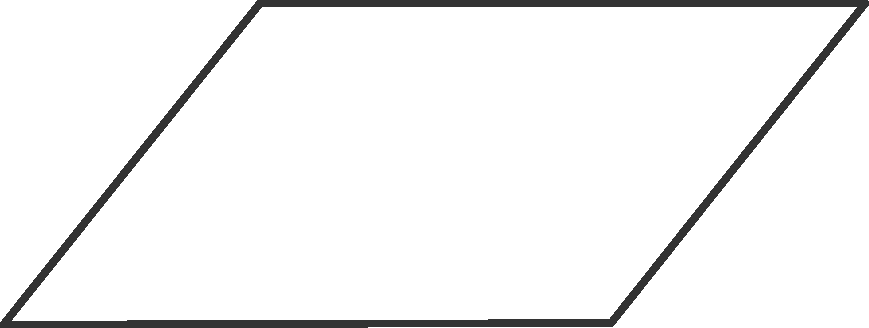
\includegraphics[width=5.5cm]{figures/curv_plan} &
      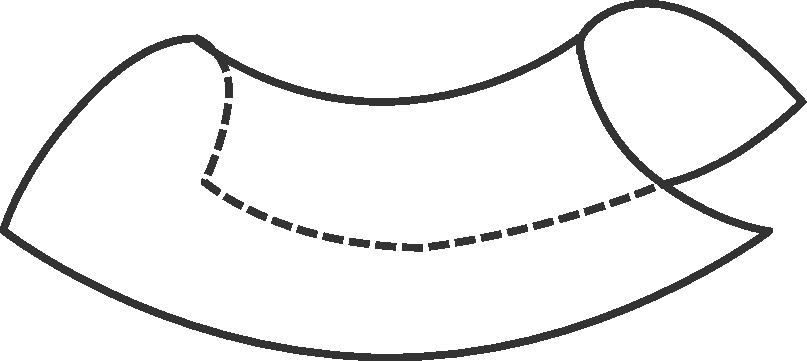
\includegraphics[width=5.5cm]{figures/curv_minimal}
      \\
      Plan &
      Surface minimale
      \\
      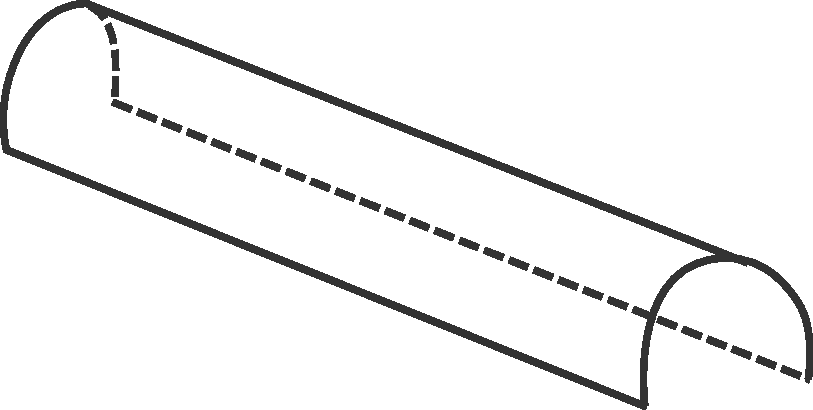
\includegraphics[width=5.5cm]{figures/curv_cylindre_conv} &
      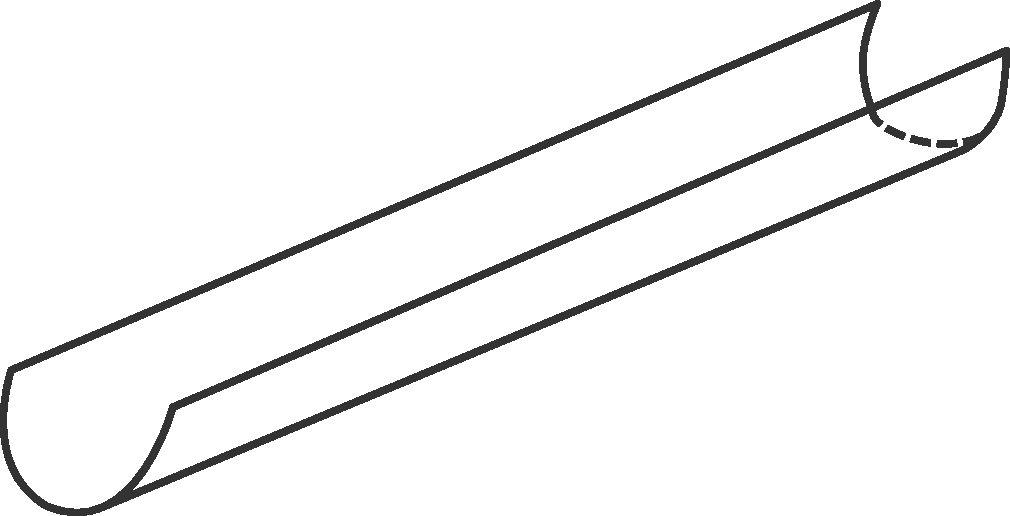
\includegraphics[width=5.5cm]{figures/curv_cylindre_conc}
      \\
      Cylindre convexe &
      Cylindre concave
      \\
      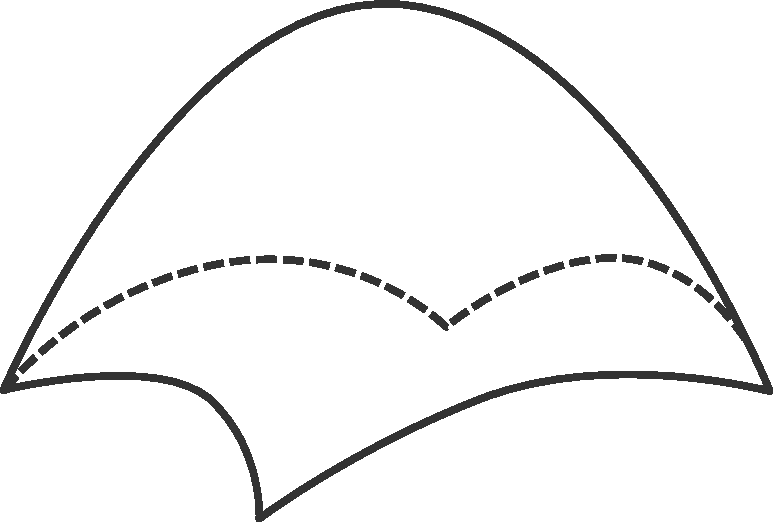
\includegraphics[width=5.5cm]{figures/curv_pic} &
      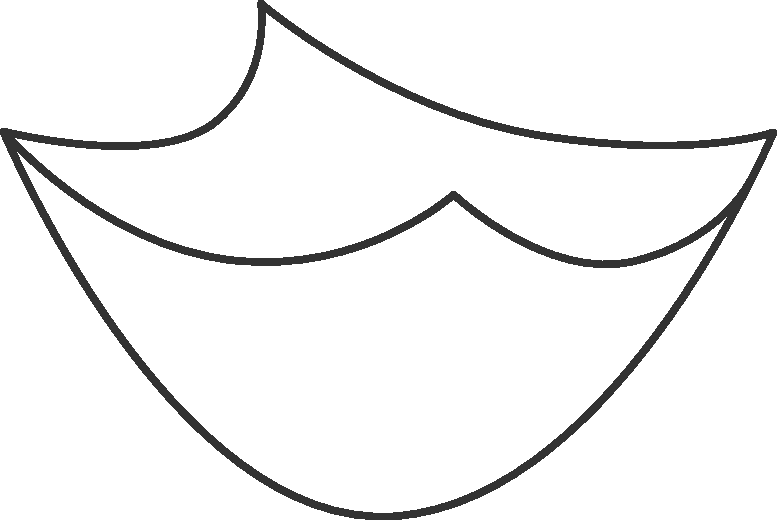
\includegraphics[width=5.5cm]{figures/curv_vallee}
      \\
      Pic &
      Vallée
      \\
      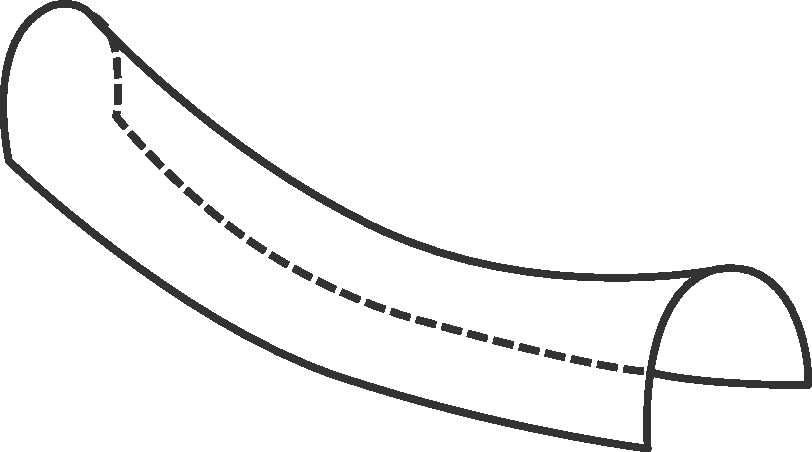
\includegraphics[width=5.5cm]{figures/curv_col_conv} &
      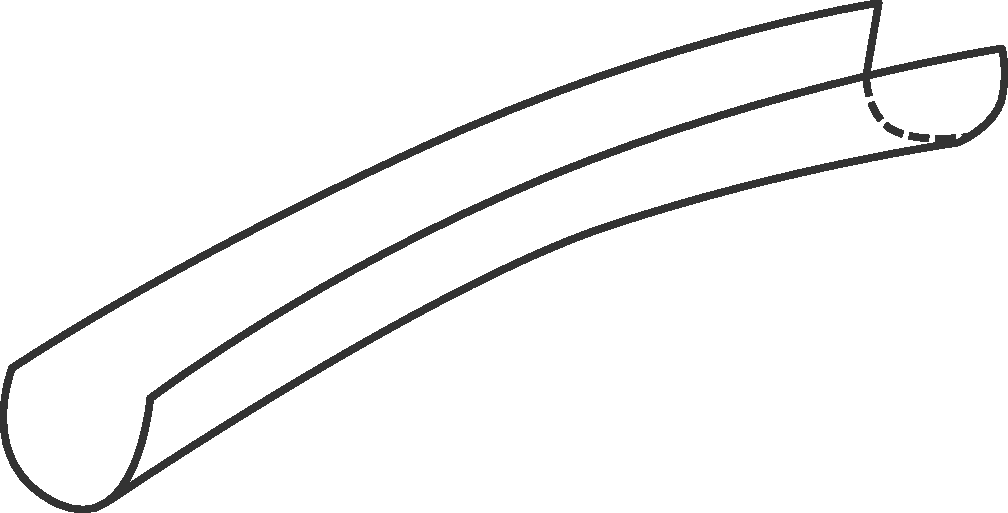
\includegraphics[width=5.5cm]{figures/curv_col_conc}
      \\
      Col convexe &
      Col concave
    \end{tabular}
    \caption[]{.\label{fig:curvature-figures}}
  \end{center}
\end{figure}


%
% \subsection{Tangente de surface}
% %
% \begin{definition}{\fakeTitle{Tangente}}
%   %
%   Nous appellons \colorize{tangente} d'une surface $\mathcal{S}$ au point $\vx$
%   %
% \end{definition}
Soit une courbe $f(\vx)$ une courbe $C^2$ paramétrée par son abscisse curviligne dans un espace de dimension $n$ :
\begin{align}
    %
    f : [0,1] &\rightarrow \R^n \nonumber\\
    \vx &\rightarrow f(\vx)
    %
\end{align}

\begin{equation}
  %
  t(\vx) = \left| \frac{df}{d\vx} \right|
  %
\end{equation}

\begin{equation}
  %
  \Curv(\vx) = \left| \frac{d^2f}{d\vx^2} \right|
  %
\end{equation}

\begin{equation}
  %
  \MeanCurv(\vx) = \frac{\PrincCurv{1} + \PrincCurv{2}}{2}
  %
\end{equation}

\begin{equation}
  %
  \GaussCurv(\vx) = \PrincCurv{1} \cdot \PrincCurv{2}
  %
\end{equation}
%
%\subsection{Courbure en dimension 2}
%
\begin{table}[ht]
\centering
\caption{My caption}
\label{my-label}
\begin{tabular}{@{}lccc@{}}
\toprule
                  & $\GaussCurv = 0$   & $\GaussCurv > 0$   & $\GaussCurv < 0$   \\ \midrule
$\MeanCurv = 0$   & plan               & indéterminé        & surface minimale   \\
$\MeanCurv > 0$   & cylindre concave   & vallée             & col concave        \\
$\MeanCurv < 0$   & cylindre convexe   & pic                & col convexe        \\ \bottomrule
\end{tabular}
\end{table}
%


\subsection{Moments géométriques}
%
Le concept mathématique des moments a beaucoup été étudié depuis plusieurs
années et trouve son champ d'application sans cesse augmenté, allant des
statistiques et mécaniques (\anglais{General moment theory}) \cite{} à la
reconnaissance de formes (\cauthors{Trier}{Trier1996} pour un survey sur la
reconnaissance de caractères, \cite{}) et la reconstruction d'objets \cite{Ghorbel2005}.
La première utilisation des moments en analyse d'images remonte à 1962 par
\cauthor{Hu}{Hu1962} pour la reconnaissance de caractères.
%
Les moments ont l'avantage d'être indépendant à l'échelle, la position et
l'orientation, en faisant un outil invariant robuste \cite{}. Nous allons tout
d'abord définir ce que sont les moments et leurs caractéristiques, pour ensuite
nous intéresser à les estimer sur des données digitales.
%
\todoJeremy{Le papier Reconstructing With Geometric Moments \cite{Ghorbel2005} est pas mal niveau intro}
%
\subsubsection{Définition et propriétés des moments géométriques}%
\label{sec:definitions-moments}
%
Une définition générale du moment géométrique (ou moment cartésien) $\Mom{p_1
\cdots p_d}$ d'ordre $p_1 \cdots p_d$ (aussi appelé le $p_1 \cdots p_d$-moment)
de $\Shape$ (de $\R^d$) peut être donnée comme :
%
\begin{equation}
  \Mom{p_1 \cdots p_d}(\Shape) \EqDef \idotsint_{\Shape} x_1^{p_1} \cdots x_d^{p_d} f(x_1 \cdots x_d) dx_1 \ldots dx_d.
\end{equation}
%
\paragraph{Moment d'ordre zéro : aire / volume}
%
Il apparaît alors que le $0\cdots0$-moment correspond à l'aire en 2D ou au
volume en 3D de $\Shape$ :
%
\begin{equation}
  \Mom{0 \cdots 0}(\Shape) \EqDef \idotsint_{\Shape} f(x_1 \cdots x_d) dx_1 \ldots dx_d.
\end{equation}
%
\paragraph{Moments du premier ordre : barycentre}
%
Les $d$ moments du premier ordre ($\Mom{1 0 \cdots 0}(\Shape)$, $\Mom{0 1 0
\cdots 0}(\Shape)$, $\cdots$, $\Mom{0 \cdots 0 1}(\Shape)$) sont généralement
utilisés pour déterminer le barycentre de la forme à analyser. Les coordonnées
du barycentre $(\overline{x_1}, \cdots, \overline{x_p})$ sont :
%
\begin{equation}
  \overline{x_1} = \frac{\Mom{1 0 \cdots 0}(\Shape)}{\Mom{0 \cdots 0}(\Shape)}, \cdots, \overline{x_p} = \frac{\Mom{0 \cdots 0 1}(\Shape)}{\Mom{0 \cdots 0}(\Shape)}.
\end{equation}
%
\paragraph{Moments du second ordre}
%
Les moments du second ordre $\Mom{p_1 \cdots p_d}(\Shape)$ avec $p_1 + \cdots +
p_2 = 2$ sont connus comme les moments d'inertie, caractérisant la géométrie des
masses de la forme. En 2D, nous en dénombrons 3 : $\Mom{2 0}(\Shape)$, $\Mom{1
1}(\Shape)$ et $\Mom{0 2}(\Shape)$, en 3D il en existe 6 :  $\Mom{2 0
0}(\Shape)$, $\Mom{0 2 0}(\Shape)$, $\Mom{0 0 2}(\Shape)$, $\Mom{1 1
0}(\Shape)$, $\Mom{0 1 0}(\Shape)$ et $\Mom{1 0 1}(\Shape)$
%
\section{Notions de bases}
\label{sec:notions-base}
%
Dans ce paragraphe, nous allons introduire les notions de bases de la géométrie
digitale comme le \colorize{pavage}. Un pavage est un ensemble de cellules
partitionnant entièrement l'espace euclidien. Il existe plusieurs types de
pavages présents dans la nature (craquement de sol sous l'effet de la chaleur,
peaux d'animaux (serpent, girafe, etc.), sol de la Chaussée des Géants
(Royaume-Uni), etc.) comme dans les constructions de l'Homme (carrelages, routes
pavées, pyramide du Louvre (Paris, France), mosaïques, vitraux, etc.), comme l'illustre la \RefFigure{fig:pavage-exemple}.


\begin{figure}[ht]
  \begin{center}
    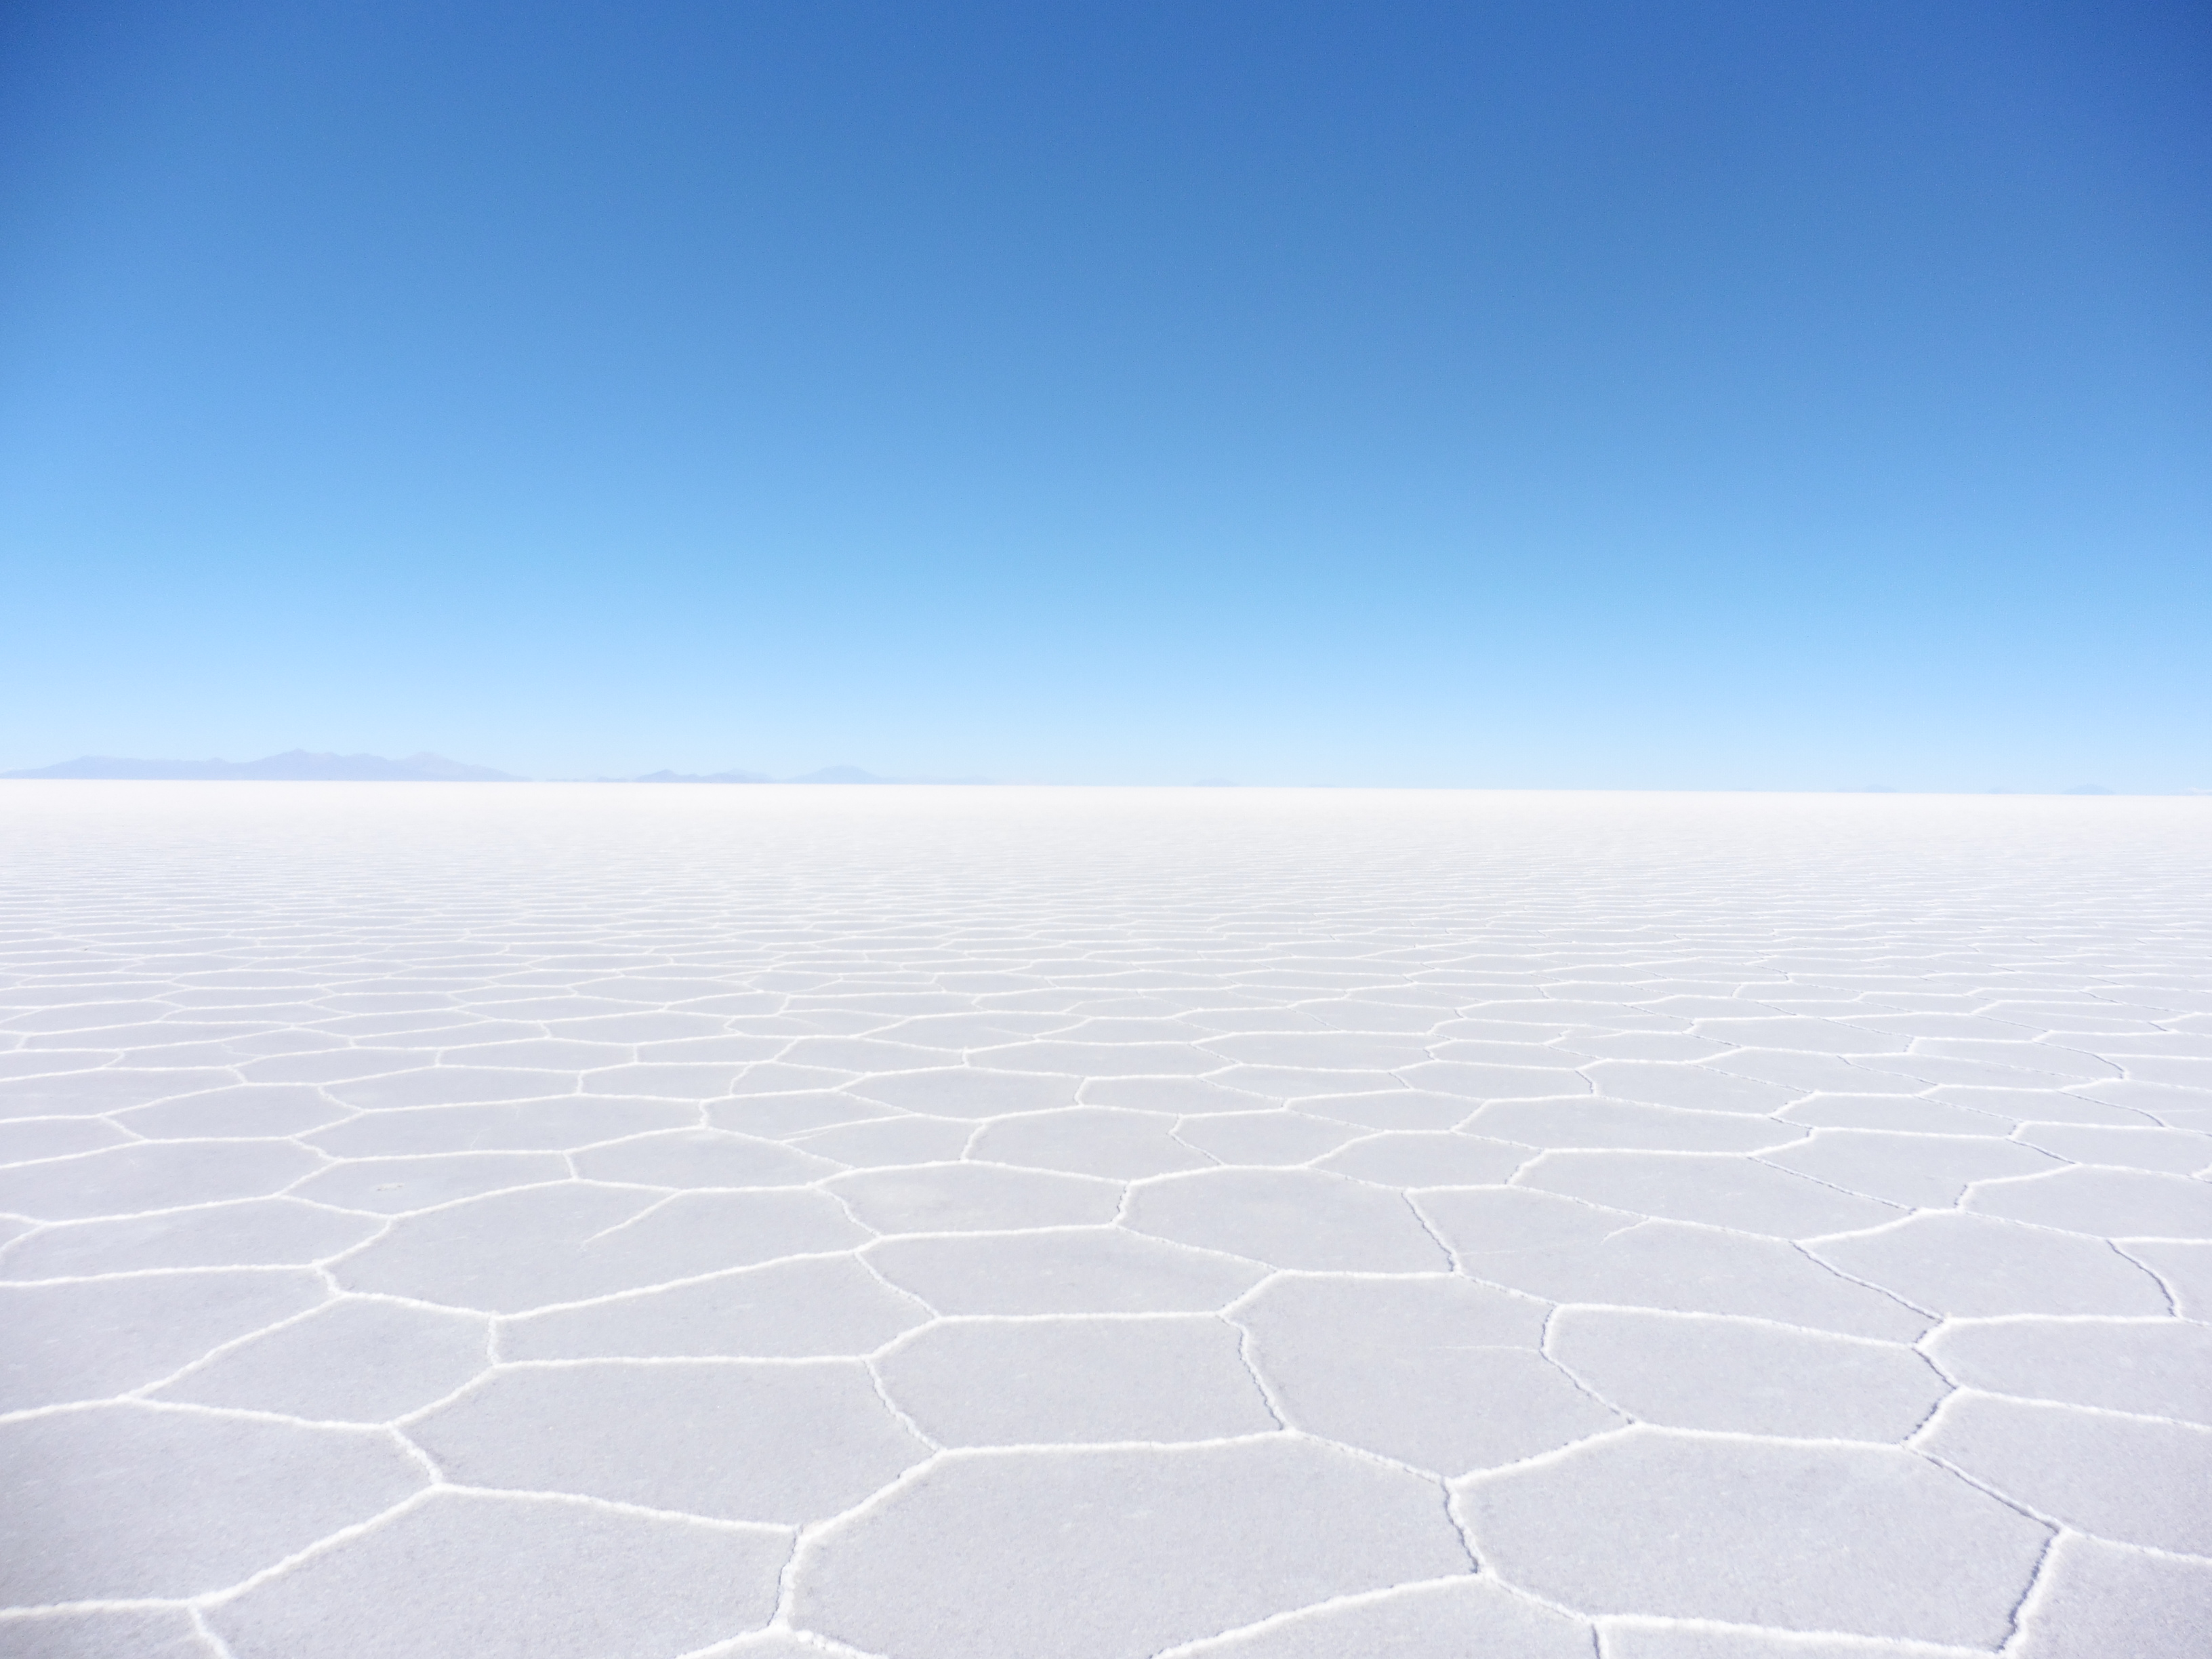
\includegraphics[width=6.8cm]{images/Notions/pavage_mer_de_sel}
    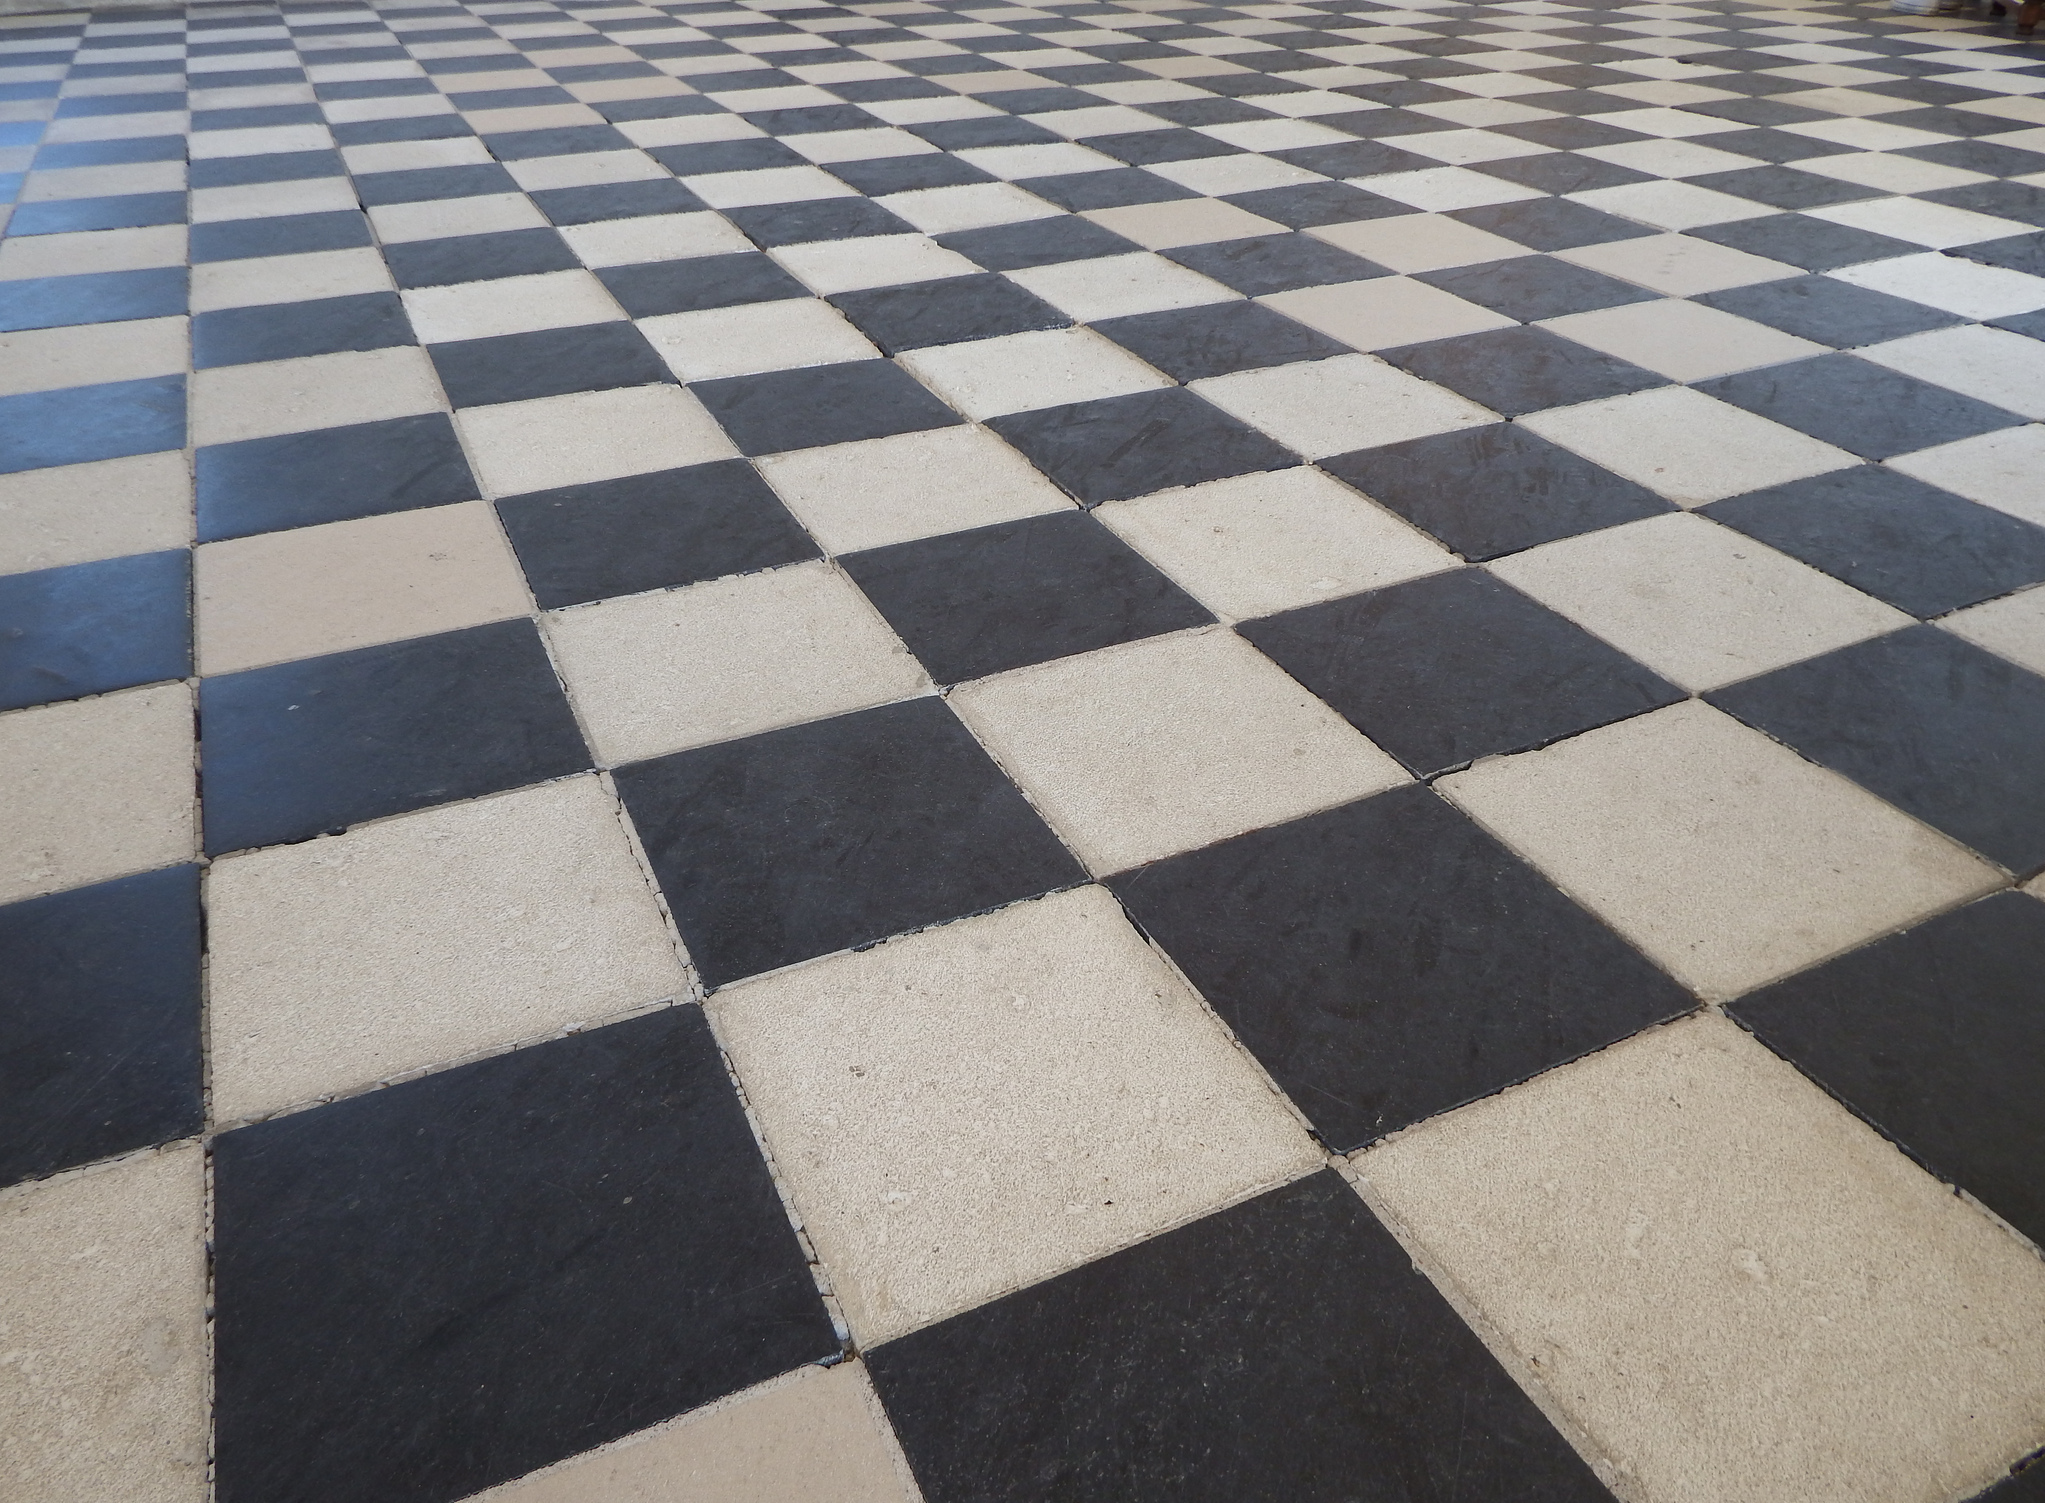
\includegraphics[width=6.8cm]{images/Notions/pavage_chateau}
    \caption[Différents pavages dans la nature ou dans les constructions humaines]{Différents pavages dans la nature ou dans les constructions humaines. \emph{De gauche à droite :} désert de sel en Bolivie \cite{pavage1}, sol d'un des châteaux de la Loire (France) \cite{pavage2}.\label{fig:pavage-exemple}}
  \end{center}
\end{figure}

Un sous-ensemble de ces pavages est le \colorize{pavage régulier}. Nous appelons
un \colorize{espace discret} un pavage régulier du plan en dimension 2 ou de
l'espace en dimension $d > 2$. Plusieurs types de pavages réguliers existent
(voir la \RefFigure{fig:pavages}), nous nous intéressons ici qu'uniquement aux
pavages discrets par carrés (ou des cubes en dimension supérieure). Ce pavage
régulier isothétique (aligné sur les axes) représente \colorize{l'espace
digital}. Ainsi, les points digitaux (\colorize{pixels} en dimension 2,
\colorize{voxels} en dimension 3) associés à cet espace sont des points de
$\Z^d$ de dimension $d$ comme nous pouvons le voir avec le graphe dual de la
\RefFigure{fig:pavage_dual}. Les coordonnées des points digitaux sont alors des
nombres entiers, rendant les calculs plus simples et stables qu'avec des
coordonnées réelles.


\begin{figure}[ht]
  \begin{center}
    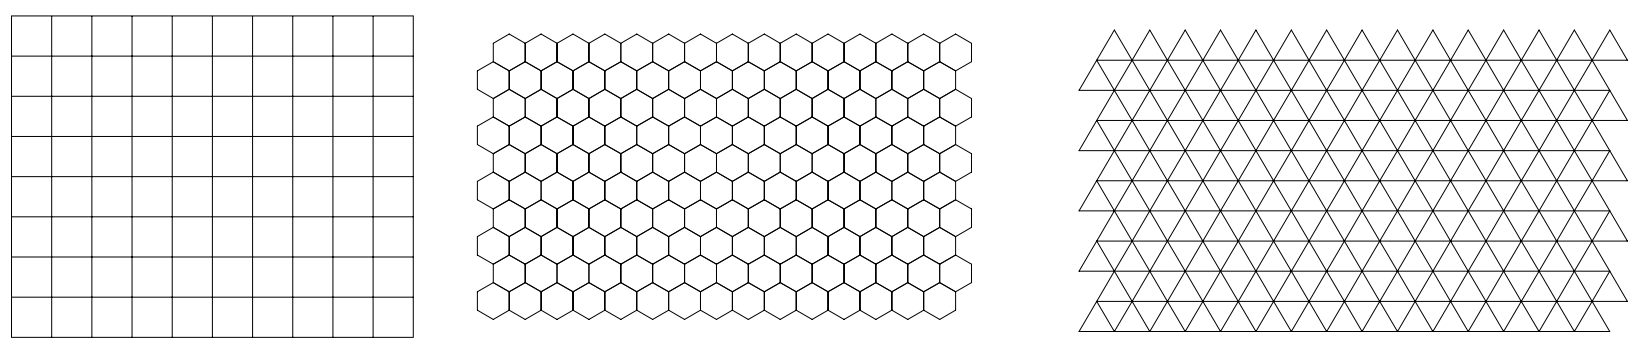
\includegraphics[width=14cm]{images/Notions/Pavages}
    \caption{Pavages 2D réguliers par carrés, hexagones et triangles.\label{fig:pavages}}
  \end{center}
\end{figure}

\begin{figure}[ht]
  \begin{center}
    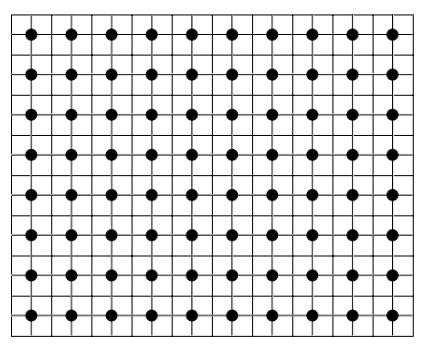
\includegraphics[width=5cm]{images/Notions/Pavage_dual}
    \caption{Dual du pavage 2D réguliers par carrés.\label{fig:pavage_dual}}
  \end{center}
\end{figure}

De ces points digitaux, nous pouvons ajouter des informations topologiques en
considérant l'espace de grille cellulaire. L'idée est de plonger l'espace
digital $\Z^n$ dans l'espace cubique cartésien afin de pouvoir représenter les
éléments entre les pixels.
%
\\
%
Ainsi, les $0$-cellules sont appelées des \colorize{pointels} (éléments de
dimension 0). Par convention, les points digitaux $\vp \in \Z^d$ sont plongés
dans des $0$-cellules.
%
\\
%
Les $1$-cellules sont appelées des \colorize{lignels} ou \anglais{linels} (éléments de dimension 1).
%
\\
%
Les $2$-cellules sont appelées des \colorize{pixels} (éléments de dimension 2).
%
\\
%
Les $3$-cellules sont appelées des \colorize{voxels} (éléments de dimension 3).


\begin{figure}[ht]
  \begin{center}
    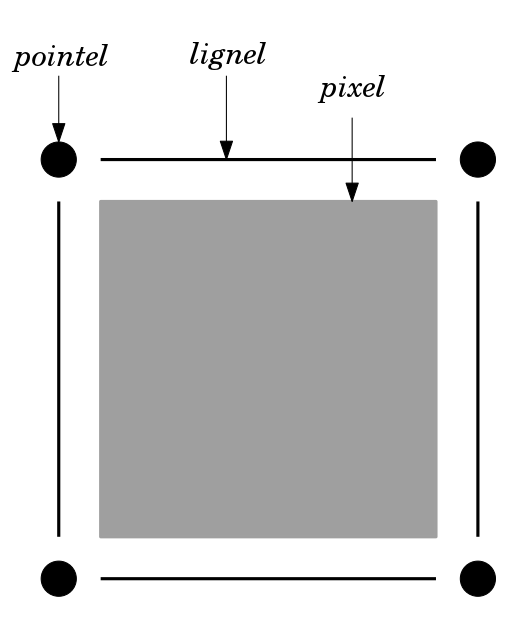
\includegraphics[width=5cm]{images/Notions/notations_topo}
    \caption{Illustration des $0$-cellules (pointels), $1$-cellules (lignels) et $2$-cellules (pixels).\label{fig:notations_topo}}
  \end{center}
\end{figure}


La \RefFigure{fig:notations_topo} illustre les pointels, lignels et pixels. Par
convention, nous nommons les $n$-cellules les \colorize{spels} (un pixel en
dimension 2), les $n-1$-cellules sont nommées les \colorize{surfels} (pour
\anglais{surface elements}).

Grâce à ces définitions, cela nous amène directement aux questions de voisinage
des points digitaux.
%
\subsection{Voisinages}
\label{sec:voisinage}
%
La relation de voisinage est une notion importante pour la définition de notre
objet digital. Le voisinage est défini en fonction de la connexité (ou de
l'adjacence) que possède une cellule digitale par rapport aux autres. Les
\RefTables{tab:adjacence2d}{tab:adjacence3d} définissent formellement ces
notions, et la \RefFigure{fig:adjacence2d} illustre la $4$-connexité et la
$8$-connexité sur un objet digital de dimension 2.

\begin{table}[ht]
  \centering
  \caption{Définition des voisinages en dimension $2$.}
  \label{tab:adjacence2d}
    \renewcommand{\arraystretch}{1.1}
  \begin{tabular}{@{}llr@{}}
    \toprule
    Adjacence & Connexité  & Caractérisation \\ \midrule
    $0$ & $4$        & $|x_1 - y_1| + |x_2 - y_2| = 1$ \\
    $1$ & $8$        & $\max(|x_1 - y_1|,|x_2 - y_2|) = 1$ \\
    \bottomrule
  \end{tabular}
\end{table}

\begin{table}[ht]
  \centering
  \caption{Définition des voisinages en dimension $3$.}
  \label{tab:adjacence3d}
    \renewcommand{\arraystretch}{1.1}
  \begin{tabular}{@{}llr@{}}
    \toprule
    Adjacence & Connexité  & Caractérisation \\ \midrule
    $0$ & $6$        & $|x_1 - y_1| + |x_2 - y_2| + |x_3 - y_3| = 1$ \\
    $1$ & $18$       & $\vx$ et $\vy$ sont 26-connexes et $|x_1 - y_1| + |x_2 - y_2| + |x_3 - y_3| \le 2$ \\
    $2$ & $26$       & $\max(|x_1 - y_1|,|x_2 - y_2|,|x_3 - y_3|) = 1$ \\
    \bottomrule
  \end{tabular}
\end{table}

\begin{figure}[ht]
  \begin{center}
    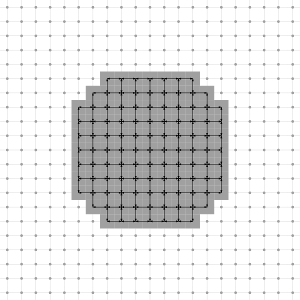
\includegraphics[width=6.8cm]{images/Notions/DiskWithAdj4}
    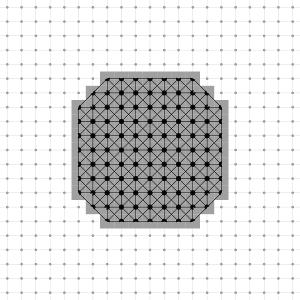
\includegraphics[width=6.8cm]{images/Notions/DiskWithAdj8}
    \caption{Illustation du voisinage en dimension 2.\label{fig:adjacence2d}}
  \end{center}
\end{figure}


Pour résumer, en dimension 2 :
%
\begin{itemize}
  %
  \item la $4$-connexité (ou $1$-adjacence) est la relation de voisinage par les arêtes;
  \item la $8$-connexité (ou $0$-adjacence) est la relation de voisinage par les arêtes et les sommets.
  %
\end{itemize}
%
De même, en dimension 3 :
%
\begin{itemize}
  %
  \item la $6$-connexité (ou $2$-adjacence) est la relation de voisinage par les faces;
  \item la $18$-connexité (ou $1$-adjacence) est la relation de voisinage par les faces et les arêtes.
  \item la $26$-connexité (ou $0$-adjacence) est la relation de voisinage par les faces, les arêtes et les sommets.
  %
\end{itemize}



La notion de voisinage est alors importante. En effet, en fonction de la
connexité de l'espace digital, différentes composantes connexes peuvent être
extraites comme le montre la \RefFigure{fig:connexite}.

\begin{figure}[ht]
  \begin{center}
    
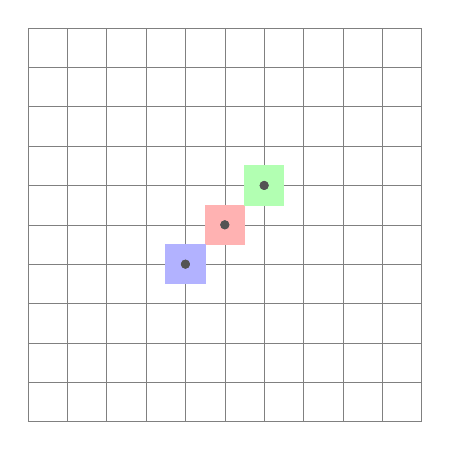
\begin{tikzpicture}[x=0.5cm,y=0.5cm]
  % colors
  \definecolor{kGreen}{rgb}{0.0,0.59,0.0}
  \definecolor{kOrange}{rgb}{1.0,0.59,0.0}
  \definecolor{kGrey}{rgb}{0.33,0.33,0.33}
  % grids
  \draw[help lines,step=0.5cm] (0,0) grid (10,10);
  % shape

  \draw[color=red!30!white,fill] (5-0.5,5-0.5) rectangle (5+0.5,5+0.5);
  \draw[color=blue!30!white,fill] (4-0.5,4-0.5) rectangle (4+0.5,4+0.5);
  \draw[color=green!30!white,fill] (6-0.5,6-0.5) rectangle (6+0.5,6+0.5);

  % gauss digitization
  \foreach \x/\y in {5/5,4/4,6/6} {
    \draw[color=kGrey,fill] (\x,\y) circle (0.5mm);
    \draw[color=kGrey,fill] (10-\x,10-\y) circle (0.5mm);
  };
\end{tikzpicture}
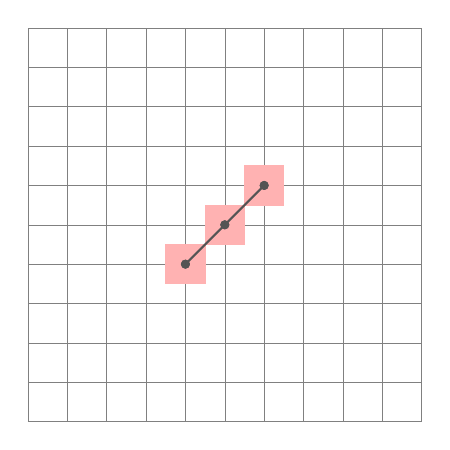
\begin{tikzpicture}[x=0.5cm,y=0.5cm]
  % colors
  \definecolor{kGreen}{rgb}{0.0,0.59,0.0}
  \definecolor{kOrange}{rgb}{1.0,0.59,0.0}
  \definecolor{kGrey}{rgb}{0.33,0.33,0.33}
  % grids
  \draw[help lines,step=0.5cm] (0,0) grid (10,10);
  % shape

  \draw[color=red!30!white,fill] (5-0.5,5-0.5) rectangle (5+0.5,5+0.5);
  \draw[color=red!30!white,fill] (4-0.5,4-0.5) rectangle (4+0.5,4+0.5);
  \draw[color=red!30!white,fill] (6-0.5,6-0.5) rectangle (6+0.5,6+0.5);

  \draw[color=kGrey,thick] (4,4) -- (5,5) -- (6,6);

  % gauss digitization
  \foreach \x/\y in {5/5,4/4,6/6} {
    \draw[color=kGrey,fill] (\x,\y) circle (0.5mm);
    \draw[color=kGrey,fill] (10-\x,10-\y) circle (0.5mm);
  };
\end{tikzpicture}

  \end{center}
  \caption[Illustration du nombre de composantes connexes en fonction de la connexité de l'espace digital.]
  %
  {Illustration du nombre de composantes connexes en fonction de la connexité de l'espace digital. \emph{À gauche :} trois composantes connexes sont extraites en $4$-connexité. \emph{À droite :} une seule composante connexe est extraites en $8$-connexité.\label{fig:connexite}}
  %
\end{figure}

%
\section{Discrétisation}
\label{sec:digitization}
%
Nous allons maintenant décrire le processus de discrétisation d'un sous-ensemble
de l'espace euclidien $\R^d$ vers un ensemble de points de l'espace digital
$\Z^d$. La formalisation de ce processus est important pour l'évaluation théorique et expérimentale des estimateurs sur les bords digitaux des objets.

Considérons une forme $\Shape$ de $\R^d$ à discrétiser en points de $\R^d$ en coordonnées entières (\cad de $\Z^d$), alors la \colorize{discrétisation de Gauss} $\DSh$ de $\Shape$ dans une grille de dimension $d$ et de résolution $h$ est :
%
\begin{equation}
  \DSh \EqDef \{ \vp \in \Z^d, (h \cdot \vp) \in \Shape \} \,,
\end{equation}
%
où $h \cdot \vp$ est le redimensionnement uniforme de $\vp$ par le facteur $h$.
Ce facteur $h$ est important car les points digitaux sont des carrés (ou cubes)
unitaires, et n'ont alors aucune information d'échelle permettant la
correspondance vers les forme euclidienne. Par exemple, la
\RefFigure{fig:scale-digital} montre deux sphères de rayons différents
discrétisés à deux échelles $h$ différentes, donnant exactement la même
discrétisation.


\begin{figure}[ht]
  \begin{center}
    
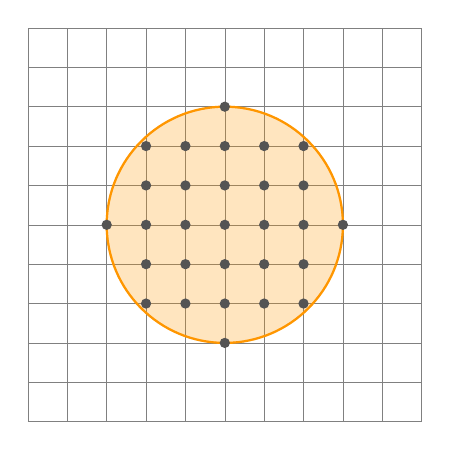
\begin{tikzpicture}[x=0.50cm,y=0.50cm]
  % colors
  \definecolor{kGreen}{rgb}{0.0,0.59,0.0}
  \definecolor{kOrange}{rgb}{1.0,0.59,0.0}
  \definecolor{kGrey}{rgb}{0.33,0.33,0.33}
  % grids
  \draw[help lines,step=1] (0,0) grid (10,10);
  \node (px) at (5,5) {};
  \draw[draw,thick,fill,color=kOrange,nearly transparent] (px) circle (3);
  \draw[draw,thick,color=kOrange] (px) circle (3);
  \foreach \x/\y in {2/5, 3/3, 3/4, 3/5, 3/6, 3/7, 4/3, 4/4, 4/5, 4/6, 4/7, 5/2, 5/3, 5/4, 5/5, 5/6, 5/7, 5/8, 6/3, 6/4, 6/5, 6/6, 6/7, 7/3, 7/4, 7/5, 7/6, 7/7, 8/5}
    \draw[draw,thick,color=kGrey,fill] (\x,\y) circle (0.1);
\end{tikzpicture}
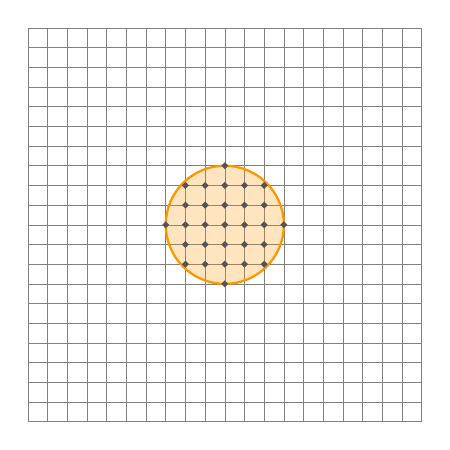
\begin{tikzpicture}[x=0.50cm,y=0.50cm]
  % colors
  \definecolor{kGreen}{rgb}{0.0,0.59,0.0}
  \definecolor{kOrange}{rgb}{1.0,0.59,0.0}
  \definecolor{kGrey}{rgb}{0.33,0.33,0.33}
  % grids
  \draw[help lines,step=0.5] (0,0) grid (10,10);
  \node (px) at (5,5) {};
  \draw[draw,thick,fill,color=kOrange,nearly transparent] (px) circle (1.5);
  \draw[draw,thick,color=kOrange] (px) circle (1.5);
  \foreach \x/\y in {3.5/5, 4/4, 4/4.5, 4/5, 4/5.5, 4/6, 4.5/4, 4.5/4.5, 4.5/5, 4.5/5.5, 4.5/6, 5/3.5, 5/4, 5/4.5, 5/5, 5/5.5, 5/6, 5/6.5, 5.5/4, 5.5/4.5, 5.5/5, 5.5/5.5, 5.5/6, 6/4, 6/4.5, 6/5, 6/5.5, 6/6, 6.5/5}
    \draw[draw,thick,color=kGrey,fill] (\x,\y) circle (0.05);
\end{tikzpicture}

  \end{center}
  \caption[Illustration de la dépendance du paramètre d'échelle $h$.]
  %
  {Illustration de la dépendance du paramètre d'échelle $h$. L'objet euclidien
  de gauche donne le même objet digital que l'objet euclidien de droite alors
  qu'ils sont à des échelles différentes.\label{fig:scale-digital}}
  %
\end{figure}

Si $\vp \in \Z^d$, alors $\Q{\vp}$ désigne le cube unitaire de dimension $d$ de
$\R^d$ centré au point $\vp$ et aligné sur les axes de $\Z^d$. Nous définissons le \colorize{$h$-cube}, \cad $\Q{\vp}$ mis à l'échelle par $h$, comme :
%
\begin{equation}
  \hQ{\vp}{h} \EqDef h\cdot \Q{\vp} \,.
\end{equation}


Ainsi, pour un ensemble digital $\DigShape \subset \Z^d$, le \colorize{corps} de $\DigShape$ est le plongement $\Body{\cdot}{h}$ de $\DigShape$ vers $\R^d$, défini comme :
%
\begin{equation}
  \Body{\DigShape}{h} \EqDef \bigcup_{\vp \in \DigShape} \hQ{\vp}{h} \,.
\end{equation}
%
En d'autres termes, $\Body{\DigShape}{h}$ est l'ensemble des cubes de dimension
$d$ appartenant à $\DigShape$, mis à l'échelle par le pas de discrétisation $h$.


Intéressons nous désormais aux bords de ces objets. Nous verrons plus tard que
certains estimateurs sont définis sur le bord de l'objet, il semble alors
important de l'étudier. Nous notons $\dS$ la \colorize{frontière} de $\Shape$,
\cad son bord topologique (en orange foncé sur la \RefFigure{fig:frontier}). La
\colorize{$h$-frontière} $\DFr{h} \DigShape$ de l'ensemble digital $\DigShape
\subset \Z^d$ est définie comme :
%
\begin{equation}
  \partial\Body{\DigShape}{h} \EqDef \partial \left( \bigcup_{\vp \in \DigShape} \hQ{\vp}{h} \right) \,.
\end{equation}
%


\begin{figure}[ht]
  \begin{center}
    
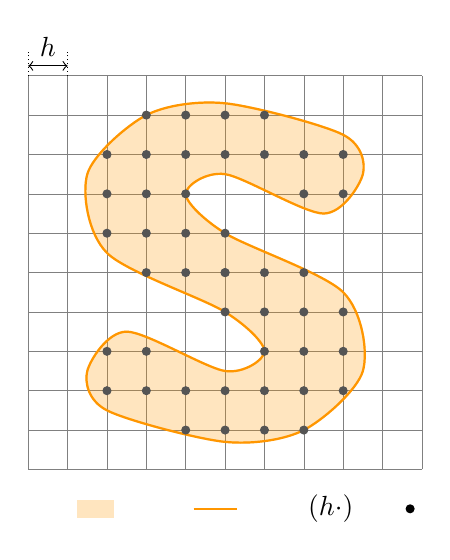
\begin{tikzpicture}[x=0.5cm,y=0.5cm]
  % colors
  \definecolor{kGreen}{rgb}{0.0,0.59,0.0}
  \definecolor{kOrange}{rgb}{1.0,0.59,0.0}
  \definecolor{kGrey}{rgb}{0.33,0.33,0.33}
  % grids
  \draw[help lines,step=0.5cm] (0,0) grid (10,10);
  % shape
  \draw[draw,thick,fill,color=kOrange,nearly transparent] plot[smooth cycle]
            coordinates{(5,9.3) (8,8.5) (8.5,7.5) (7.5,6.5) (5,7.5) (4,7) (5,6) (8,4.5) (8.5,2.5) (7,1)
                        (5,0.7) (2,1.5) (1.5,2.5) (2.5,3.5) (5,2.5) (6,3) (5,4) (2,5.5) (1.5,7.5) (3,9)} -- cycle;
  % shape boundary
  \draw[draw,thick,color=kOrange] plot[smooth cycle]
            coordinates{(5,9.3) (8,8.5) (8.5,7.5) (7.5,6.5) (5,7.5) (4,7) (5,6) (8,4.5) (8.5,2.5) (7,1)
                        (5,0.7) (2,1.5) (1.5,2.5) (2.5,3.5) (5,2.5) (6,3) (5,4) (2,5.5) (1.5,7.5) (3,9)} -- cycle;
  % gauss digitization
  \foreach \x/\y in {3/9,4/9,5/9,6/9,2/8,3/8,4/8,5/8,6/8,7/8,8/8,2/7,3/7,4/7,7/7,8/7,2/6,3/6,4/6,5/6,3/5,4/5,5/5} {
    \draw[color=kGrey,fill] (\x,\y) circle (0.5mm);
    \draw[color=kGrey,fill] (10-\x,10-\y) circle (0.5mm);
  };
  % legend
  \node at(0.5,-1) {$\Shape$};
  \node[rectangle,fill,color=kOrange,nearly transparent] at(1.7,-1) {\mbox{~~}};
  \node at(3.7,-1) {$\dS$};
  \draw[draw,thick,color=kOrange] (4.2,-1) -- (5.3,-1);
  \node at(7.8,-1) {$(h\cdot\DSh)$~~};
  \draw[color=black,fill] (9.7,-1) circle (0.5mm);
  \draw[densely dotted,black] (0,10) -- (0,10.6);
  \draw[densely dotted,black] (1,10) -- (1,10.6);
  \draw[<->,black] (0,10.25) -- (1,10.25) node[midway,above] {$h$};
\end{tikzpicture}
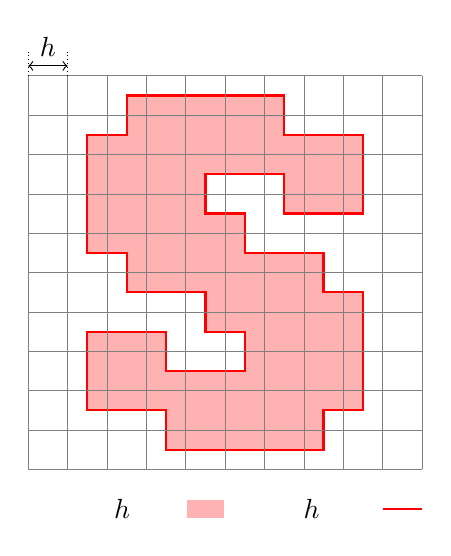
\begin{tikzpicture}[x=0.5cm,y=0.5cm]
  % colors
  \definecolor{kGreen}{rgb}{0.0,0.59,0.0}
  \definecolor{kOrange}{rgb}{1.0,0.59,0.0}
  \definecolor{kGrey}{rgb}{0.33,0.33,0.33}
  % QhZ
  \foreach \x/\y in {3/9,4/9,5/9,6/9,2/8,3/8,4/8,5/8,6/8,7/8,8/8,2/7,3/7,4/7,7/7,8/7,2/6,3/6,4/6,5/6,3/5,4/5,5/5} {
    \draw[color=red!30!white,fill] (\x-0.5,\y-0.5) rectangle (\x+0.5,\y+0.5);
    \draw[color=red!30!white,fill] (10-\x-0.5,10-\y-0.5) rectangle (10-\x+0.5,10-\y+0.5);
  };
  % \partial_h X
  \draw[color=red,thick] (2.5,9.5) -- (6.5,9.5) -- (6.5,8.5) -- (8.5,8.5) -- (8.5,6.5) -- (6.5,6.5)
                             -- (6.5,7.5) -- (4.5,7.5) -- (4.5,6.5) -- (5.5,6.5) -- (5.5,5.5) -- (7.5,5.5)
                             -- (7.5,4.5) -- (8.5,4.5) -- (8.5,1.5) -- (7.5,1.5) -- (7.5,0.5) -- (3.5,0.5)
                             -- (3.5,1.5) -- (1.5,1.5) -- (1.5,3.5) -- (3.5,3.5) -- (3.5,2.5) -- (5.5,2.5)
                             -- (5.5,3.5) -- (4.5,3.5) -- (4.5,4.5) -- (2.5,4.5) -- (2.5,5.5) -- (1.5,5.5)
                             -- (1.5,8.5) -- (2.5,8.5) -- cycle;
  % grids
  \draw[help lines,step=0.5cm] (0,0) grid (10,10);
  \node at(2.5,-1) {$\Body{\DSh}{h}$~~};
  \node[color=red!30!white,fill] at(4.5,-1) {\mbox{~~}};
  \node at(7.2,-1) {$\Bd{\Body{\DSh}{h}}$}; %% := \partial \hCube{h} \GD{h}X$};
  \draw[color=red,thick] (9,-1) -- (10,-1);
  \draw[densely dotted,black] (0,10) -- (0,10.6);
  \draw[densely dotted,black] (1,10) -- (1,10.6);
  \draw[<->,black] (0,10.25) -- (1,10.25) node[midway,above] {$h$};
\end{tikzpicture}

  \end{center}
  \caption{Illustration d'une forme euclidienne $\Shape$, de sa frontière $\dS$, du corps de sa discrétisation de Gauss $\Body{\DSh}{h}$ et sa $h$-frontière $\partial\Body{\DSh}{h}$.\label{fig:frontier}}
\end{figure}


La \RefFigure{fig:frontier} montre une forme euclidienne $\Shape \subset \R^2$
(en orange pâle) et sa frontière $\dS$ (en orange foncé), ainsi que
$\Body{\DSh}{h}$ le corps de la discrétisation de Gauss de $\Shape$ avec le pas
de discrétisation $h$ (en rouge pâle) et sa $h$-frontière
$\partial\Body{\DSh}{h}$ (en rouge foncé). Les points $\vp \in \DSh$ remis à
l'échelle par le facteur $h$ sont en noir sur la figure de gauche.


Comme nous pouvons le voir sur la \RefFigure{fig:frontier}, la $h$-frontière de
$\DSh$ est un sous-ensemble de dimension $(d-1)$ de $\R^d$ qui est proche
de $\partial \Shape$. Pour certaines preuves mathématiques cette notion de
proximité est essentielle. Une correspondance précise entre les points $\vx \in
\dS$ et $\hat{\vx}\in \partial\Body{\DSh}{h}$ est alors nécessaire.
%
\\
%
Pour un forme $\Shape \subset \R^d$, l'\colorize{axe médian} $MA(\dS)$ de $\dS$
est le sous-ensemble de $\R^d$ dans lequel tous les points sont les plus proche
d'au moins deux points de $\dS$. Le \colorize{reach} de $\Shape$ est la borne
inférieure de la distance entre $\dS$ et son axe médian. Les formes à reach
positif ont leur courbures principales bornées par $\pm 1 / \Reach{\Shape}$.
Nous définissons la \colorize{projection orthogonale} $\ProjX{\Shape}$ comme la
correspondance de $\Shape \setminus MA(\dS)$ vers $\dS$ qui associe tout point
vers son point le plus proche de $\dS$.
%
\\
%
Dans notre cas, nous souhaitons restreindre cette projection au domaine
$\partial\Body{\DSh}{h}$ afin de définir la correspondance $\Proj$ de la
$h$-frontière $\partial\Body{\DSh}{h}$ vers le bord topologique $\dS$ de
$\Shape$. Cette projection est nommée la \colorize{projection inverse} ou
\anglais{back-projection} \cite{Lachaud2006} :
%
\begin{definition}{\fakeTitle{Projection inverse $\Proj$ \cite{Lachaud2006}}}
\label{def:projection}
%
  Pour tout forme 2D $\Shape$ à reach positif, pour $0 < h \le \Reach{\Shape}$,
  soit $\NormalDir(\Shape,\vx,l)$ le segment centré au point $\vx$, aligné le
  long de la normale au point $\vx$ et de demi-longueur $l$ Alors la
  \colorize{projection inverse} $\Proj$ est définie comme :
  %
  \begin{align}
    \Proj: \partial\Body{\DigShape}{h} &\rightarrow \dS, \nonumber \\
    \hat{\vx} &\mapsto \vx=\Proj(\hat{\vx}) \,,
  \end{align}
  %
  où $\vx$ est le seul point tel que $\hat{\vx} \in
  \NormalDir(\Shape,\vx,\frac{\sqrt{2}}{2}h)$.
%
\end{definition}
%
Le \RefLemmaFake{B.9}{Lachaud2006} nous indique que la correspondance $\Proj$
n'introduit aucune ambiguïté et est surjectif, et le
\RefLemmaFake{B.10}{Lachaud2006} que cette correspondance est continue. La
\RefFigure{fig:backproj} nous montre (en rouge) la projection de tout point
$\hat{\vx} \in \partial\Body{\DSh}{h}$ vers des points $\vx \in \dS$. Alors,
nous pouvons conclure que les bords $\partial\Body{\DSh}{h}$ et $\dS$ ont une
distance de Hausdorff inférieure ou égale à $\frac{\sqrt{2}}{2}h$. De plus, la
projection $\ProjX{\Shape}$ est continue sur $\R^d \setminus MA(\dS)$, donc
également sur $\partial\Body{\DSh}{h}$ avec un $h$ adéquat.
%
\section{Convergence asymptotique d'estimateurs locaux et globaux}
\label{sec:multigrid-convergence-estimator}
%
Maintenant que le processus de discrétisation est défini, nous allons nous intéresser aux propriétés de convergence asymptotique des estimateurs de quantités géométriques. Tout d'abord, nous pouvons distinguer deux types de quantités géométriques : les quantités « locales » et les quantités « globales » :
%
\begin{definition}{\fakeTitle{Quantités géométriques locales et globales}}
  \label{def:global-quantity}
  %
  Une quantité géométrique est dite « locale » lorsqu'elle est définie
  localement sur le bord de la forme. Une quantité géométrique est dite «
  globale » lorsqu'elle est définie pour la forme.
  %
\end{definition}
%
Il apparaît alors clairement que, par exemple, le volume d'une forme est une
quantité géométrique « globale », tandis que la normale, la courbure ou encore
la tangente sur sa surface sont des quantités géométriques dites « locales ».


Alors nous pouvons nous définir ce qu'est la \colorize{convergence asymptotique
d'estimateurs} de quantités géométriques (locales et globales). La notion de
convergence asymptotique, introduite en $1983$ par \cauthor{Serra}{Serra1983},
est un critère important permettant d'évaluer et de comparer des estimateurs
digitaux. L'idée principale est, pour une forme euclidienne $\Shape$ donnée,
d'évaluer l'erreur entre une quantité géométrique de $\Shape$ et la quantité
géométrique digitale estimée sur la discrétisation de $\Shape$, à plusieurs
échelles de discrétisation. Le comportement attendu est alors que si nous
raffinons l'objet digital (\cad que le pas de discrétisation diminue, donnant
ainsi un objet digital plus proche de la forme euclidienne), l'erreur
d'estimation doit diminuer.


Ainsi, définissons $\hat{E}(\DSh,h)$ (\respp $\hat{E}(\DSh,\hat{\vx},h)$) un
estimateur de quantité géométrique globale (\resp locale) sur $\DSh$ la
discrétisation (de Gauss, voir le \RefSection{sec:digitization}) de la forme
$\Shape$ au pas de discrétisation $h$. La version locale est définie sur un
point $\hat{\vx}$ le bord digital $\partial\Body{\DSh}{h}$ de la discrétisation
de la forme $\Shape$ au pas de discrétisation $h$.


Alors, nous pouvons étudier la convergence asymptotique de ces estimateurs
(\RefDefinitionFake{2.10}{Klette2004}) :
%
\begin{definition}{\fakeTitle{Convergence asymptotique d'un estimateur digital de quantité géométrique globale}}
  \label{def:multigrid-convergence-global}
  %
  Un estimateur digital de quantité géométrique globale $\hat{E}$ d'une quantité géométrique
  $E$ \colorize{converge asymptotiquement} pour une famille de formes $\Shapes$ si
  et seulement si pour toute forme $\Shape \in \Shapes$, il existe un pas de
  discrétisation $h_0 > 0$ tel que l'estimation de $\hat{E}(\DSh,h)$
  soit défini pour tout $0 < h < h_0$,
  %
  \begin{equation}
    | \hat{E}(\DSh,h) - E(\Shape) | \le \tau_{\Shape}(h) \,,
  \end{equation}
  %
  où $\tau_{\Shape}: \R^{+*} \rightarrow \R^+$, désignant l'erreur d'estimation
  de la quantité géométrique pour le pas de discrétisation $h$, a une limite
  nulle à $0$. Cette fonction définie la vitesse de convergence de $\hat{E}$
  vers $E$ sur $\Shape$. La convergence est dite \colorize{uniforme} pour
  $\Shape$ lorsque toutes les valeurs de $\tau_{\Shape}$ sont bornées (borne
  supérieure) par une fonction $\tau_\Shape$ indépendante de $\vx \in \dS$ avec
  une limite nulle à $0$.
  %
\end{definition}
%
Lorsqu'une quantité géométrique est « locale », nous avons besoin de connaître
explicitement la correspondance entre $\dS$ et $\Boundary{\Body{\DSh}{h}}$. Un
estimateur local digital estime la quantité géométrique sur les points de la
$h$-frontière de l'ensemble digital. En d'autre termes, l'estimation se fait en
tout point situé à entre les pixels internes de l'objet digital et les pixels
externes.
%
\begin{definition}{\fakeTitle{Convergence asymptotique d'un estimateur digital de quantité géométrique locale}}
  \label{def:multigrid-convergence-local}
  %
  Un estimateur digital de quantité géométrique locale $\hat{E}$ d'une quantité géométrique
  $E$ \colorize{converge asymptotiquement} pour une famille de formes $\Shapes$ si
  et seulement si pour toute forme $\Shape \in \Shapes$, il existe un pas de
  discrétisation $h_0 > 0$ tel que l'estimation de $\hat{E}(\DSh,\hat{\vx},h)$
  soit défini en tout point $\hat{\vx} \in \hBd{h} \Shape$ avec $0 < h < h_0$,
  et pour tout $\vx \in \dS$,
  %
  \begin{equation}
    \forall \hat{\vx} \in \partial\Body{\DSh}{h} \text{~avec~} \| \hat{\vx} -\vx\|_\infty
    \le h, \quad | \hat{E}(\DSh,\hat{\vx},h) - E(\Shape,\vx) | \le \tau_{\Shape,\vx}(h) \,,
  \end{equation}
  %
  où $\tau_{\Shape,\vx}: \R^{+*} \rightarrow \R^+$ a une limite
  nulle à $0$. Cette fonction définie la vitesse de convergence de $\hat{E}$
  vers $E$ au point $\vx$ de $\Shape$. La convergence est dite
  \colorize{uniforme} pour $\Shape$ lorsque toutes les valeurs de
  $\tau_{\Shape,\vx}$ sont bornées (borne supérieure) par une fonction
  $\tau_\Shape$ indépendante de $\vx \in \dS$ avec une limite nulle à $0$.
  %
\end{definition}


Concrètement, cela revient à prouver que l'erreur d'estimation est en $O(h^a)$,
avec $a$ une constante. Alors, lorsque $h$ tend vers $0$, l'erreur tend
également vers $0$. Nous nous intéressons dans cette thèse à la
\colorize{convergence asymptotique uniforme} de nos estimateurs, en d'autres
mots il s'agit l'erreur dans le pire des cas de nos estimateurs.
%
\section{Droites digitales standard, segments digitaux, arcs de cercle digitaux}%
\label{sec:segments}
%
Nous allons maintenant nous intéresser à la définition de primitives digitales.
Ces primitives seront estimées et, grâce à leurs bonnes propriétés
mathématiques, pourront utilisées par la suite comme point d'entré d'estimateurs
de quantités différentielles comme la courbure (ce que nous verrons dans le
\RefChapitre{sec:estimators}).


La primitive la plus basique à reconnaître est sans nul doute la droite. Alors
nous devons définir ce qu'une droite représente dans l'espace digital et ce
n'est pas trivial à cause de la discrétisation de la forme. Définissons tout
d'abord une \colorize{droite digitale standard} (ou droite $4$-connexe), et
ainsi le \colorize{segment digital} :
%
\begin{definition}{\fakeTitle{Droite digitale standard et segment digital (« \anglais{Digital Straight Segment} ») \cite{Reveilles1991}}}
  \label{def:DSS}
%
  L'ensemble de points $(p_1,p_2) \in \Z^2$ satisfaisant $\mu \le ap_1 - bp_2 <
  \mu + |a| + |b|$, avec $a$, $b$ et $\mu$ des nombres entiers, est appelé une
  \colorize{droite digitale standard} avec comme pente $a/b$ et comme décalage
  $\mu$. Tout sous ensemble de pixels connectés d'une droite digitale standard
  est un \colorize{segment digital} (ou « \anglais{DSS} »).
%
\end{definition}


Ainsi, de cette définition, nous pouvons en extraire les \colorize{segments
maximaux} ainsi que le \colorize{faisceau de segments maximaux} :
%
\begin{definition}{\fakeTitle{Segments maximaux et faisceau de segments maximaux \cite{Lachaud2007}}}
  \label{def:MDSS}
%
  Les pointels composant le bord digital $\BdZ{\DigShape}$ d'une forme
  $\DigShape \subset \Z^2$ forme un contour $4$-connecté. Cela nous permet de
  les dénombrer consécutivement par $(\vp_i)_{i={0\ldots n-1}}$. Une séquence de
  pointels $(\vp_i, \ldots, \vp_j)$ (dont l'indice est modulo $n$) est un
  \colorize{segment maximal} (ou « \anglais{MDSS} ») sur $\BdZ{\DigShape}$ si c'est
  un DSS qui ne peut s'étendre dans aucun sens (en avant ou en arrière) en
  restant un DSS.
  %
  \\
  %
  Plus formellement, $(\vp_i, \ldots, \vp_j)$ est un segment maximal sur $\BdZ{\DigShape}$ \ssi :
  \begin{itemize}
    \item $(\vp_i, \ldots, \vp_j)$ est un DSS sur $\BdZ{\DigShape}$,
    \item $(\vp_{i-1}, \ldots, \vp_j)$ n'est pas un DSS sur $\BdZ{\DigShape}$,
    \item $(\vp_i, \ldots, \vp_{j+1})$ n'est pas un DSS sur $\BdZ{\DigShape}$,
  \end{itemize}
  %
  Pour un pointel $\vp \in \BdZ{\DigShape}$ donné, le \emph{faisceau de segments maximaux} à $\vp$ est l'ensemble
  des segments maximaux de $\BdZ{\DigShape}$ contenant $\vp$.
%
\end{definition}


Il parait alors essentiel d'étudier le comportement asymptotique de ces
primitives afin de pouvoir les exploiter au sein d'estimateurs auxquels nous
voulons prouver la convergence. \cauthors{Lachaud}{lachaud2006HDR} et
\cauthors{de Vieilleville}{deVieilleville2007} se sont alors intéressés sur les
propriétés asymptotiques des longueurs des segments maximaux sur des formes
convexe suffisamment lisse de dimension $2$ :
%
\begin{lemma}{\fakeTitle{Lois asymptotiques des segments maximaux}}
  \label{lem:law-length-MDSS}
  %
  Soit $\Shape$ une forme convexe de $\R^2$, avec un bord $C^3$ à
  courbure bornée non nulle. La longueur discrète des segments maximaux de
  $\BdZ{\DigShape}$ pour $\DigShape = \DSh$ suit les règles suivantes :
  %
  \begin{itemize}
    %
    \item le \colorize{plus court des segments maximaux} a une borne inférieure en
    $\Omega(h^{-\frac{1}{3}})$;
    %
    \item le \colorize{plus long des segments maximaux} a une borne supérieure en
    $O(h^{-\frac{1}{2}})$;
    %
    \item la \colorize{longueur moyenne des segments maximaux} $L_D({\DigShape})$, est
    bornée par :
    %
    \begin{equation}
      \label{eq:lengthMS}
      \Theta(h^{-\frac{1}{3}}) \le L_D( {\DigShape} ) \le \Theta(h^{-\frac{1}{3}} \log \left(\frac{1}{h}\right))\;.
    \end{equation}
  \end{itemize}
  %
\end{lemma}


\begin{figure}[ht]{
    \begin{center}
    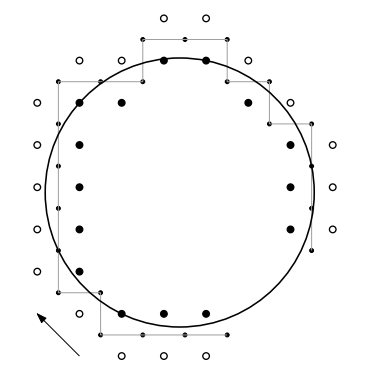
\includegraphics[height=6cm]{images/Notions/DCA}
    \end{center}}
    \caption[Arc de cercle digital.]{Arc de cercle digital (Figure~1.22 de \cite{Roussillon2009}).\label{fig:dca-figure}}
\end{figure}


L'arc de cercle est une autre primitive intéressante à étudier. En effet,
puisque la courbure est l'inverse du rayon du cercle osculateur du bord d'un
objet, le reconnaître permettrait d'approcher cette valeur. Définissons alors
\colorize{l'arc de cercle digital} (voir la \RefFigure{fig:dca-figure}) :
%
\begin{definition}{\fakeTitle{Arcs de cercle digitaux}}
  \label{def:digital-circular-arc}
  %
  Soit $\Shape$ une forme convexe de $\R^2$, avec un champ de courbure continue.
  Le contour digital $\BdZ{\DigShape}$ pour $\DigShape = \DSh$ est un \colorize{arc de
  cercle digital} (\anglais{DCA}) si et seulement s'il existe un cercle euclidien
  qui sépare les points intérieurs à $\BdZ{\DigShape}$ des points digitaux
  extérieurs de $\BdZ{\DigShape}$ (voir \RefFigure{fig:dca-figure}).
  %
  \\
  %
  Un arc de \colorize{cercle digital est maximal} (\anglais{MDCA}) si et seulement s'il ne
  peut être étendu dans aucune direction.
  %
\end{definition}


Nous verrons dans le chapitre suivant des estimateurs utilisant ces primitives
digitales pour estimer la courbure. Nous allons également proposer un estimateur
digital de courbure tirant parti des segments maximaux.
%
\section{Estimateurs digitaux d'aire, de volume, de moments, de positionnement de surface}
%
Nous avons vu dans le \RefSection{sec:geo-diff} certaines quantités
différentielles, comme l'aire, le volume ou encore les moments. Ces quantités
différentielles peuvent être très facilement estimées sur des surfaces
digitales, le calcul intégral pouvant se limiter à compter des points digitaux.
Nous allons ici détailler l'estimation digitale d'aire, de volume et des moments
sur des surfaces digitales provenant de la littérature, ainsi que leurs
convergence.
%
\subsection{Aire et volume digitaux en dénombrant les points digitaux}
\label{sec:AreaByCounting}
%
Une façon simple de calculer l'aire ou le volume d'une forme digitale consiste à
compter le nombre de points digitaux appartenant à la forme. Plus formellement,
pour tout sous-ensemble $\DigShape \subset \Z^2$, l'estimateur digital d'aire au pas
de discrétisation $h$ est défini par :
%
\begin{equation}
  \AreaC(\DigShape, h) \EqDef h^2 \MCard(\DigShape)
\end{equation}
%
En dimension $3$, nous noterons l'estimateur digital de volume au pas de
discrétisation $h$ :
%
\begin{equation}
  \VolC(\DigShape, h) \EqDef h^3 \MCard(\DigShape)
\end{equation}
%
Maintenant, si ce sous-ensemble digital $\DigShape$ provient de la discrétisation de
formes euclidiennes $\Shape$, nous voulons que l'estimation du volume devienne
meilleure lorsque le pas de discrétisation $h$ se raffine (voir
\RefSection{sec:notion:multigridconvergence}). Il est connu depuis
\nauthor{Gauss} et \nauthor{Dirichlet} que cette façon d'estimer l'aire donne
des résultats de convergence asymptotique sur les formes $\Shape$ convexes
finies de $\R^2$ :
%
\begin{equation}
  \label{eq:AreaByCountingConv}
  \AreaC(\DigF{\Shape}{h},h) = \Area(\Shape) + O(h^\beta),
\end{equation}
%
avec $\beta = 1$ dans le cas général \cite{Klette2000}, et peut être optimisé à
$\beta = \frac{15}{11} - \epsilon$ avec $\epsilon > 0$ (arbitrairement petit)
lorsque le bord de l'objet est $C^3$ à courbure non nulle \cite{Huxley1990}.
De mêmes résultats ont été proposés en 3D :
%
\begin{equation}
  \label{eq:VolumeByCountingConv}
  \VolC(\DigF{\Shape}{h},h) = \Vol(\Shape) + O(h^\gamma),
\end{equation}
%
avec $\gamma = 1$ dans le cas général \cite{Kratzel1988}, et peut être amélioré à
$\gamma=\frac{243}{158}$ lorsque le bord est lisse \cite{Guo2010}.
%
En dimension 2, les objets non convexes suivent les mêmes règles tant que
$\Shape$ peut être exprimé comme une somme ou une différence de régions convexes
bornées par des courbes fermées simples \cite{Huxley1996}. Ces résultats
précédents restent valides chaque fois que le bord de la forme peut être
décomposé en nombre fini de morceaux convexes (ou convexe $C^3$ à courbure non
nulle pour les bornes améliorées).
%
\subsection{Moments géométriques digitaux en dénombrant les points digitaux}
\label{sec:MomentsByCounting}
%
Comme pour l'aire ou le volume précédemment, il est très simple de calculer les
moments sur des données digitales. En effet, il suffit de sommer les valeurs des
points digitaux de la forme et de remettre à l'échelle suivant le pas de
discrétisation $h$. Plus formellement, pour tout sous-ensemble $\DigShape$ de
$\Z^d$, le $p_1 \cdots p_d$-moment digital de $\DigShape$ au pas de
discrétisation $h$ est défini par :
%
\begin{equation}
  \DMom{p_1 \cdots p_d}{h}(\DigShape) \EqDef h^{d + p_1 + \cdots + p_d} \sum_{(z_1,\ldots,z_d) \in \DigShape} z_1^{p_1} \cdots z_d^{p_d} f(z_1^{p_1} \cdots z_d^{p_d}).
\end{equation}
%
Il est à noter que $f(z_1 \cdots z_d)$ est tout le temps égal à $1$ lorsque
$(z_1,\ldots,z_d) \in \DigShape$, $0$ sinon, nous pouvons alors l'enlever de
l'équation :
%
\begin{equation} \label{eq:MomentsByCounting-def}
%
  \DMom{p_1 \cdots p_d}{h}(\DigShape) \EqDef h^{d + p_1 + \cdots + p_d} \sum_{(z_1,\ldots,z_d) \in \DigShape} z_1^{p_1} \cdots z_d^{p_d}.
%
\end{equation}
%
Ainsi, le $0$-moment digital de $\DigShape$ correspond au volume digital de
$\DigShape$, \cad $\AreaC(\DigShape,h)$ lorsque $d = 2$ et $\VolC(\DigShape,h)$
lorsque $d \geq 3$.
%
Nous souhaitons alors borner l'erreur entre les moments de $\Shape$ et
l'estimation des moments digitaux de la discrétisation de $\Shape$ comme
fonction du pas de discrétisation $h$. \cauthors{Klette}{Klette2000} ont
démontré la convergence de cet estimation des moments avec une vitesse de
convergence dépendante de l'ordre du moment $\sigma = p_1 + \cdots + p_d$ :
%
\begin{equation} \label{eq:MomentsByCounting-conv}
%
  \DMom{p_1 \cdots p_d}{h}(\DigF{\Shape}{h},h) = \Mom{p_1 \cdots p_d}(\Shape) + O(h^{\mu_{\sigma}}).
%
\end{equation}
%
avec $\mu_{\sigma} \ge 1$ dans le cas général (\todoJeremy{expliciter}). Cette
borne peut être améliorer lorsque la courbure gaussienne n'est pas nulle :
\cauthors{Krätzel}{Kratzel1991} obtiennent $\mu_0=\frac{38}{25}-\epsilon$ et
\cauthors{Müller}{Muller1999} obtiennent $\mu_0 = \frac{66}{43}-\epsilon$.
%
%\section{Enveloppes convexes}
%
\section{Conclusion}
%
\todoInlineJeremy{Conclusion notions à faire}
